\documentclass{beamer}
\mode<presentation>
{
  \usetheme{Warsaw}
  \setbeamertemplate{navigation symbols}{}
  \setbeamertemplate{caption}[numbered]
}

\usepackage[english]{babel}
\usepackage[T1]{fontenc}
\usepackage[utf8]{inputenc}
\usepackage{lmodern}

\title[Bot do gry w Szachy]{Bot dla gry w Szachy}
\author[K. Wiśniewski]{\textbf {Krzysztof Wiśniewski} \\ dr Maciej Gębala, prof. uczelni}
\institute[]{
  Politechnika Wrocławska\\
  Wydział Informatyki i Telekomunikacji\\
  Informatyka Algorytmiczna \\
}
\date{Styczeń 2025}

\begin{document}

\begin{frame}
  \titlepage
\end{frame}

%  \section{Wstęp}\label{sec:wstep}

\begin{frame}{Wstęp}

    \begin{block}{Silniki szachowe}
        Silnik szachowy
    \end{block}

    \begin{block}{Cel pracy}
        \begin{enumerate}
            \item Stworzenie silnika
            \item Testowanie silnika
        \end{enumerate}
    \end{block}

\end{frame}
  \section{Tworzenie silnika szachowego}\label{sec:tworzenie silnika szachowego}

\begin{frame}{Reprezentacja szachownicy i generowanie ruchów}

    \begin{columns}
        \column{0.45\textwidth}
        \begin{block}{Reprezentacja szachownicy}
            \begin{itemize}
                \item Tablica pól szachowych
                \item Tablice bitowe bierek
            \end{itemize}
            \centering {
                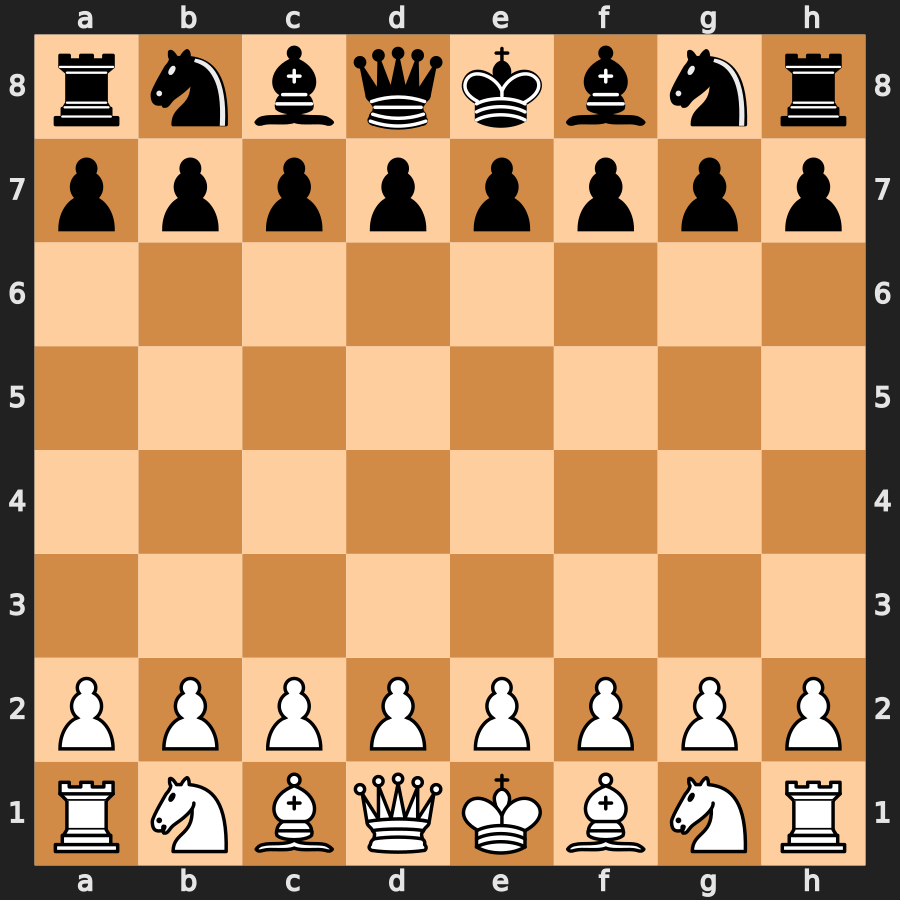
\includegraphics[width=0.8\textwidth]{rysunki/pozycja_startowa}
            }
        \end{block}
        \column{0.55\textwidth}

        \begin{block}{Generowanie ruchów pionów}
                    $moves & = empty$ \\
                    $moves & = moves \wedge (pionki_w\ll16)$ \\
                    $moves & = moves \wedge (empty\ll8)$ \\
                    $moves & = moves \wedge rank4$ \\
        \end{block}

        \begin{block}{Hyperbola Quintessence}
            $linia = (o-2r) \oplus \Bigr[( o'-2r')\Bigl]'$
        \end{block}

    \end{columns}
\end{frame}

\begin{frame}{Wyszukiwanie i ewaluacja}
    \begin{columns}
        \column{0.5\textwidth}
        \begin{block}{Charakterystyka szachów}
            \begin{enumerate}
                \item Gra dwuosobowa
                \item Gra o sumie stałej
                \item Postać ekstensywna
                \item Gra skończona
                \item Gra o doskonałej informacji
            \end{enumerate}

        \end{block}

        \begin{alertblock} {Gra ściśle konkurencyjna}
            Aby uzyskać maksymalną wypłatę, gracz dąży do tego, by~zminimalizować sumę wypłat
            przeciwnika.
        \end{alertblock}

        \column{0.5\textwidth}

        \centering {
            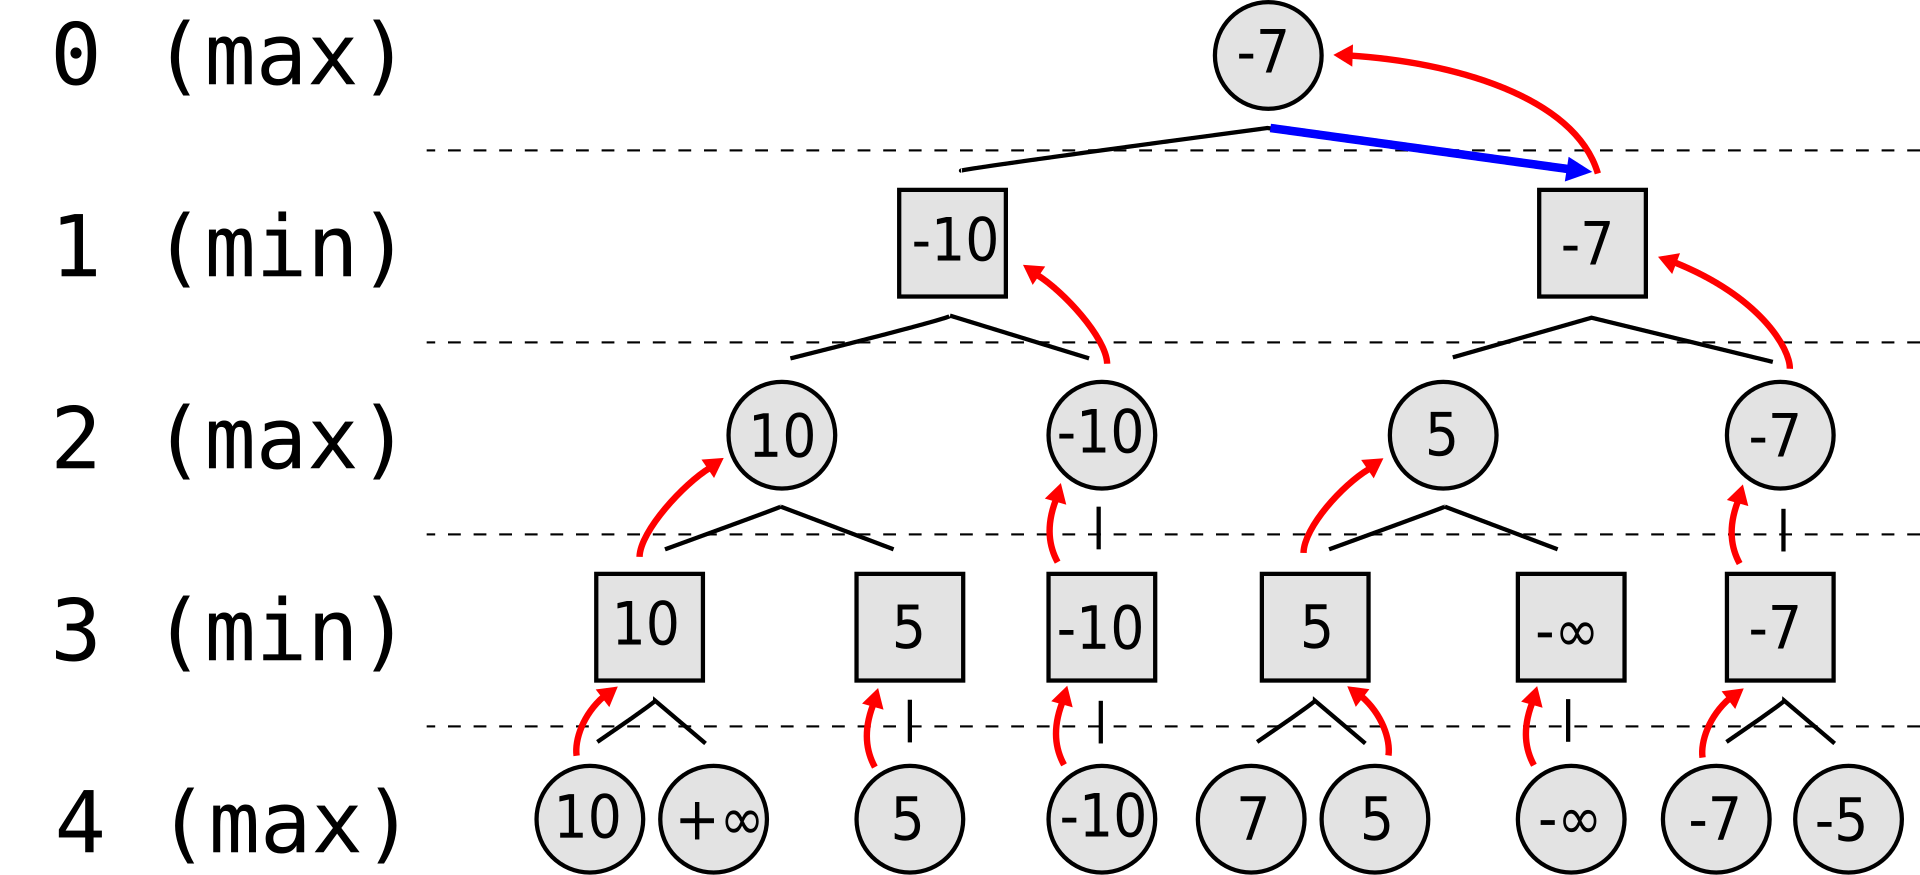
\includegraphics[width=1\textwidth]{rysunki/minimax}
        }

        \begin{block}{Ocena heurystyczna}
            \begin{itemize}
                \item Ocena stanu gry
                \item Wartość bierek
            \end{itemize}
        \end{block}

    \end{columns}
\end{frame}
  \section{Ulepszenia}\label{sec:ulepszenia-dla-silnika}

\begin{frame}{Ulepszenia dla algorytmów wyszukiwania - I}

    \begin{columns}
        \column{0.5\textwidth}
            \begin{block}{Alfa-Beta cięcie}
                \begin{table}[] \tiny
                \centering
                \label{tab:alfa-beat-limit}
                \renewcommand{\arraystretch}{1.5}
                \begin{tabular}{|c|c|c|}\hline
                $n$ & $({b_{f}})^{n}$ & $b_{f}^{\lceil \frac{n}{2} \rceil} + b_{f}^{\lfloor \frac{n}{2} \rfloor} - 1$\\ \hline\hline

                $1$ & $35$ & $35$\\ \hline
                $2$ & $1\,225$ & $69$\\ \hline
                $3$ & $42\,875$ & $1\,259$\\ \hline
                $\vdots$ & $\vdots$ & $\vdots$\\ \hline
                $10$ & $\simeq2,76 * 10^{15}$ & $\simeq1,05 * 10^{8}$\\ \hline

                \end{tabular}
                \end{table}
            \end{block}
        \column{0.5\textwidth}
            \begin{block}{Wyniki rozgrywek}
                \centering {
                    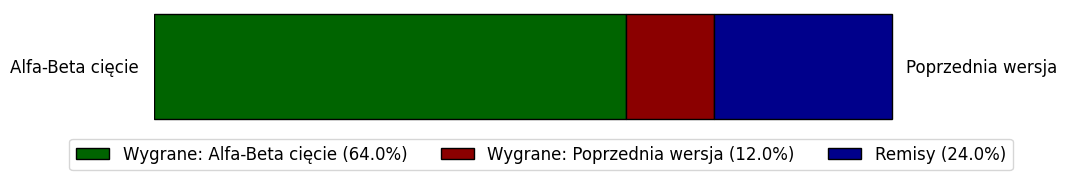
\includegraphics[width=1\textwidth]{rysunki/wyniki-alfa-beta}
                    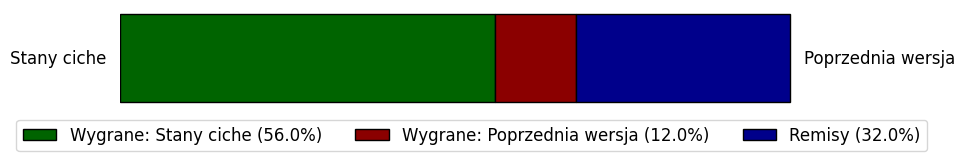
\includegraphics[width=1\textwidth]{rysunki/wyniki-stany-ciche}
                    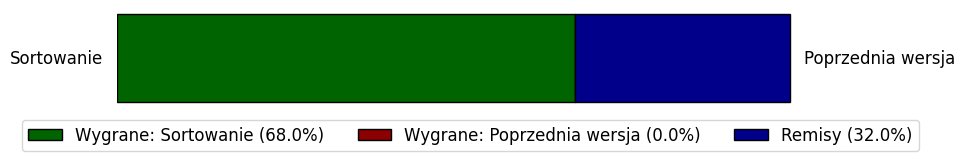
\includegraphics[width=1\textwidth]{rysunki/wyniki-sortowanie}
                    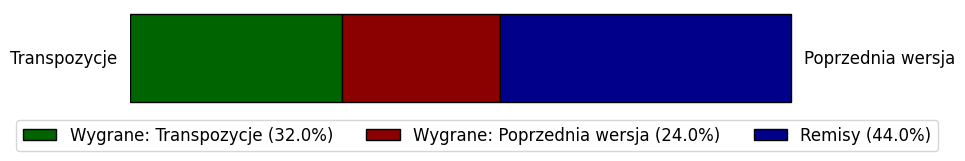
\includegraphics[width=1\textwidth]{rysunki/wyniki-transpozycje}
                }
            \end{block}

    \end{columns}

    \begin{block}{Lista zaimplementowanych ulepszeń algorytmów wyszukiwania}
        \centering {
            \small{Biblioteka otwarć, Alfa-Beta cięcie, Ewaluacja stanów cichych, Sortowanie ruchów, Tabela transpozycji, Okno estymacji.}
        }
    \end{block}



\end{frame}

\begin{frame}{Ulepszenia dla algorytmów wyszukiwania - II}
    \begin{flushright}
        \begin{table}[h!]
            \centering
            \resizebox{\textwidth}{!}{
                \begin{tabular}{|c|r|r|r|r|r|r|r|}
                    \hline
                    Start pos & Stockfish & Wersja podstawowa & Alfa-beta & Quiescence & Move ordering & Estimation & Transposition \\
                    \hline
                    1. & $20$ & $20$ & $20$ & $20$ & $20$ & $20$ & $20$ \\
                    2. & $400$ & $400$ & $186$ & $194$ & $214$ & $214$ & $214$ \\
                    3. & $8\,902$ & $8\,902$ & $2\,262$ & $2\,279$ & $2\,360$ & $2\,741$ & $2\,360$ \\
                    4. & $197\,281$ & $197\,281$ & $20\,596$ & $23\,119$ & $20\,428$ & $23\,597$ & $17\,481$ \\
                    5. & $4\,865\,609$ & $4\,865\,609$ & $223\,840$ & $225\,836$ & $173\,183$ & $199\,062$ & $123\,575$ \\
                    6. & $119\,060\,324$ & $119\,060\,324$ & $3\,349\,766$ & $1\,606\,833$ & $1\,019\,119$ & $1\,245\,427$ & $615\,267$ \\
                    7. & $3\,195\,901\,860$ & xxx & $20\,668\,442$ & $19\,449\,096$ & $7\,934\,005$ & $9\,078\,322$ & $3\,923\,917$ \\
                    8. & $84\,998\,978\,956$ & xxx & $275\,274\,306$ & $183\,000\,753$ & $57\,778\,837$ & $70\,097\,202$ & $23\,360\,242$ \\
                    \hline
                \end{tabular}
            }
            \label{tab:engine-comparison-1}
        \end{table}
        \begin{columns}
            \column{0.5\textwidth}
                \centering {
                    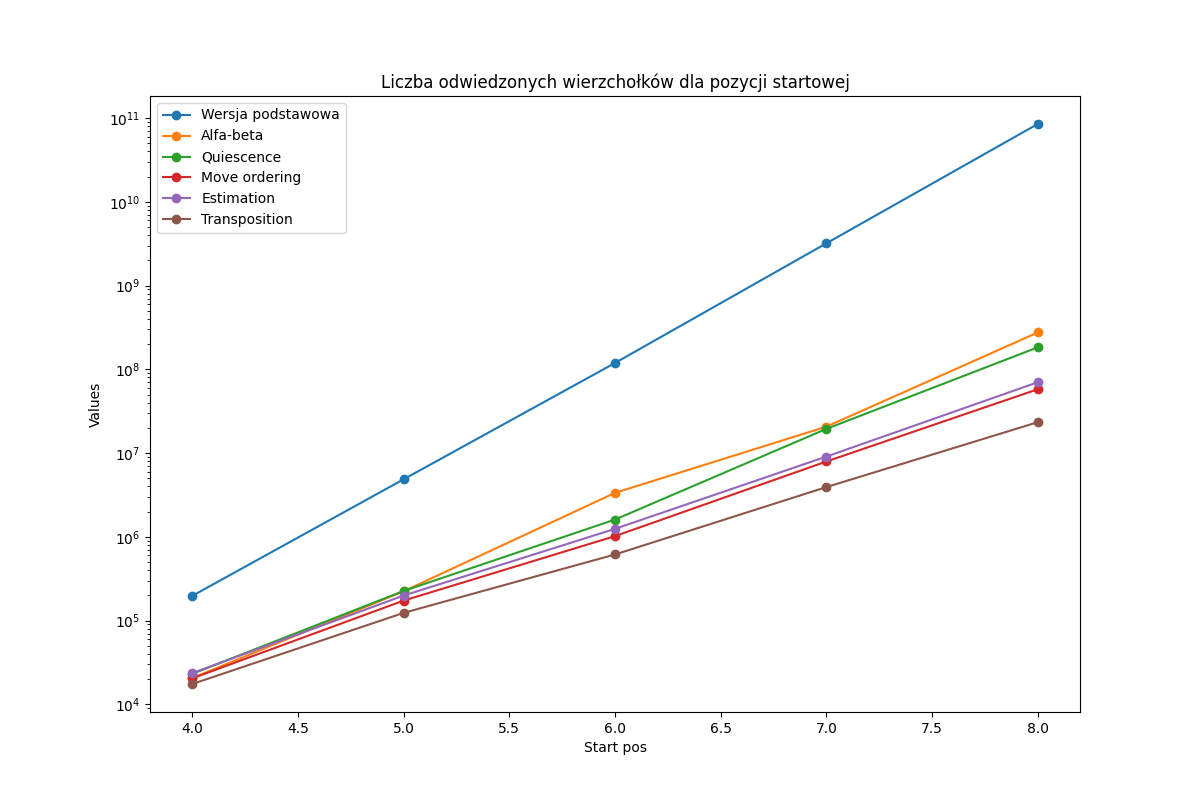
\includegraphics[width=1\textwidth]{rysunki/visited-chart}
                }
            \column{0.5\textwidth}
                \centering {
                    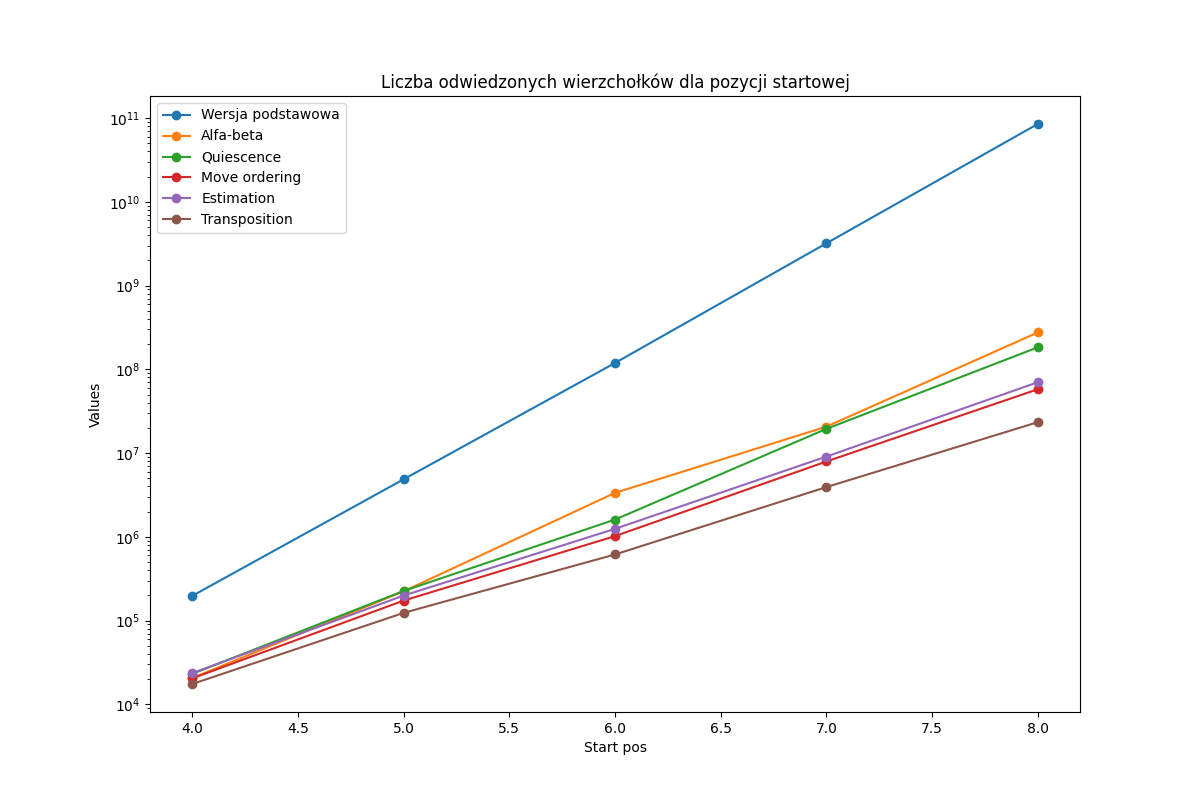
\includegraphics[width=1\textwidth]{rysunki/visited-chart}
                }
        \end{columns}
    \end{flushright}
\end{frame}

\begin{frame}{Ulepszenia dla oceny heurystycznej}

    \begin{columns}
        \column{0.5\textwidth}
            \begin{block}{Tablice figur}
                    \centering {
                        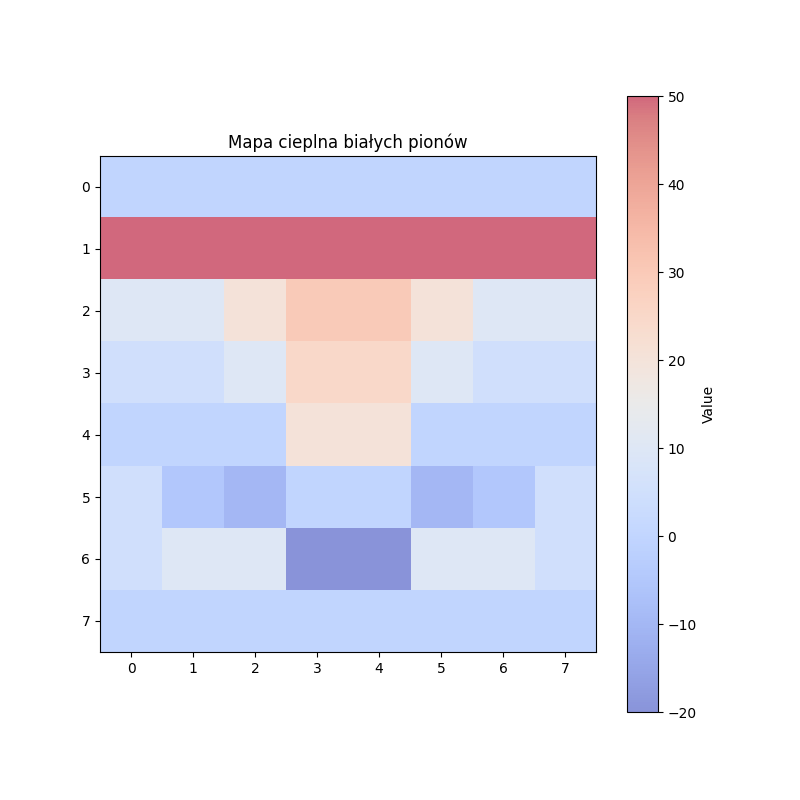
\includegraphics[width=0.6\linewidth]{rysunki/bialePiony}
                    }
            \end{block}
        \column{0.5\textwidth}
            \begin{block}{Wyniki rozgrywek}
                \centering {
                    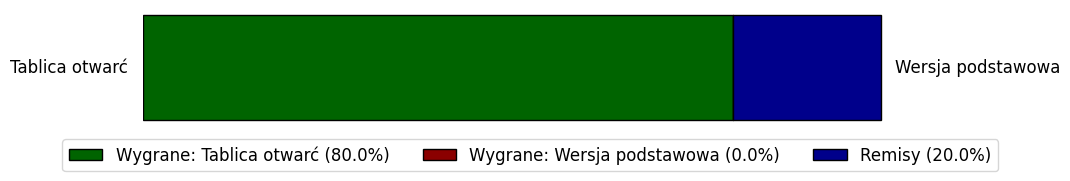
\includegraphics[width=1\linewidth]{rysunki/wyniki-tablica}
                    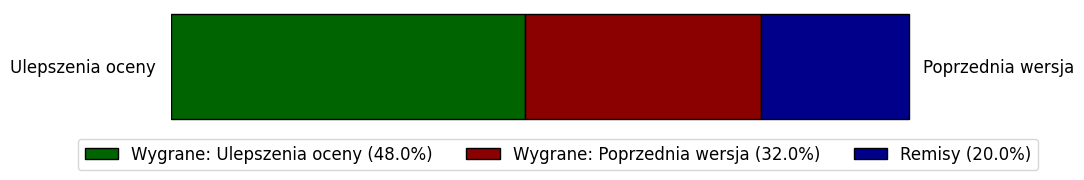
\includegraphics[width=1\linewidth]{rysunki/wyniki-full-eval}
                }
            \end{block}
    \end{columns}

    \begin{block}{Lista zaimplementowanych ulepszeń oceny heurystycznej}
        \centering {
            Tablice figur, Ochrona króla, Struktura pionów, Moment gry.
        }
    \end{block}
\end{frame}
  \section{Testowanie}\label{sec:testowanie-sily-silnika}

\begin{frame}{Testowanie siły silnika}
    \begin{columns}
        \begin{column}{0.5\textwidth}
            \begin{block}{Platforma Lichess}
                \begin{enumerate}
                    \item \textbf{Ranking silnika} – $1\,617$ELO
                    \item \textbf{Ranking przeciwnika} – $1\,625.85$ELO
                    \item \textbf{Wśród graczy} – $38$\%
                    \item \textbf{Ruchów na grę} – $43.41$
                    \item \textbf{Czas ruchu} – $5.65$ sekundy
                    \item \textbf{Wygranych} – $41.1$\%
                    \item \textbf{Remisów} – $16.9$\%
                    \item \textbf{Strata do ruchu optymalnego} – $45.29$ ACPL
                \end{enumerate}
            \end{block}
        \end{column}
        \begin{column}{0.5\textwidth}
            \begin{block}{Sekwencyjny test probabilistyczny}
                $H_{0}:p=p_{0}$, $H_{1}:p=p_{1}$ \\

                $S_{i}=S_{i-1}+\log \Lambda _{i}$
                \begin{itemize}
                    \item $S_{i} \le \alpha$ : $H_{0}$
                    \item $S_{i} \ge \beta$ : $H_{1}$
                    \item $S_{i} \in (\alpha, \beta)$ : brak decyzji
                \end{itemize}

                \centering {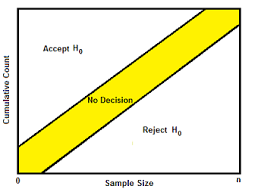
\includegraphics[width=0.7\linewidth]{rysunki/sprt}}
            \end{block}
        \end{column}
    \end{columns}
\end{frame}
  \section{Dalsze kierunki rozwoju}\label{sec:dalsze-kierunki-rozwoju}

\begin{frame}{Dalsze możliwości rozwoju}

    \begin{block}{Wybrane przykłady}
        \begin{enumerate}
            \item Algorytm genetyczny
            \item Dynamiczne sortowanie ruchów
            \item Sieć neuronowa
            \item Połączenie z LLM
        \end{enumerate}
    \end{block}

    \begin{alertblock}
        \centering{
            \textbf{Dziękuję za uwagę!}
        }
    \end{alertblock}
\end{frame}

\end{document}